% Lecture Template for ME3050-001-002-Tristan Hill - Spring 2020
% Dynamics Modeling and Controls
% Time Response - Lecture 3

% I am finally converting my stuff to BEAMER

% Document settings

%\documentclass{beamer}                  % for presentation ?
\documentclass[handout]{beamer}  % for handout ?
\usepackage{beamerthemesplit}
\usepackage{amsmath}
\usepackage{listings}
\usepackage{multicol}
\usepackage{framed}
\usepackage{amssymb}



\beamertemplateballitem

\definecolor{TTUpurple}{rgb}{0.3098, 0.1607, 0.5176} % TTU Purple (primary)
\definecolor{TTUgold}{rgb}{1.0000, 0.8666, 0.0000} % TTU Gold (primary)

\setbeamercolor{palette primary}{bg=TTUpurple,fg=TTUgold}
\setbeamercolor{palette secondary}{bg=black,fg=TTUgold}
\setbeamercolor{palette tertiary}{bg=black,fg=TTUpurple}
\setbeamercolor{palette quaternary}{bg=TTUgold,fg=black}
\setbeamercolor{structure}{fg=TTUpurple} % itemize, enumerate, etc
\setbeamercolor{section in toc}{fg=TTUpurple} % TOC sections

%\DeclareSymbolFont{bbold}{U}{bbold}{m}{n}
%\DeclareSymbolFontAlphabet{\mathbbold}{bbold}

%\newcommand{\bbfamily}{\fontencoding{U}\fontfamily{bbold}\selectfont}
%\DeclareMathAlphabet{\mathbbold}{U}{bbold}{m}{n}

%\usefonttheme{professionalfonts}

\newcommand{\vspccc}{\vspace{6mm}\\} % large vertical space
\newcommand{\vspcc}{\vspace{4mm}\\}   % medium vertical space
\newcommand{\vspc}{\vspace{2mm}\\}     % small vertical space

\newcommand{\hspcccc}{\hspace{10mm}} % large horizontal space
\newcommand{\hspccc}{\hspace{6mm}} % large horizontal space
\newcommand{\hspcc}{\hspace{4mm}}   % medium horizontal space
\newcommand{\hspc}{\hspace{2mm}}     % small horizontal space


\newcommand{\Lagr}{\mathcal{L}} % lagrangian

\newcommand{\LNUM}{1} %Lecture number 1

\newcommand{\secondtitle}{Frequency Response of First Order Systems}% second line of the title of this presentation , aka the topic of this lecture

\title{Frequency Response - Lecture \LNUM}
\author{ME3050 - Dynamics Modeling and Controls} % original formatting from Mike Renfro, September 21, 2004

\date{April  19, 2020}

\begin{document}

\lstset{language=MATLAB,basicstyle=\ttfamily\small,showstringspaces=false}

% Title page1 
\frame{\titlepage \center\textbf{\secondtitle}\vspcc}


% Section 0: Outline
\frame{

\large \textbf{Lecture \LNUM - \secondtitle} \vspc

 \begin{itemize}

	\item Introduction to Chapter 9\vspc % Section 1: The Step Input

	\item Review Complex Numbers\vspc        % Section 2
	
	\item Frequency Response of First Order Systems\vspc %Section 3

	\item The Bode Plot\vspace{2mm} % Section 4

\end{itemize}

}


%Section 1: Introduction to Chapter 9
\section{Introduction to Chapter 9}

\subsection{Harmonic Input Function}
\frame{
\frametitle{Harmonic Input Function}

\large The term {\bf frequency response} is used to describe a system's response to a periodic input. Frequency response analysis focuses on a system's response to {\it harmonic} input such as sines and cosines. The input (forcing) function is written below.\vspcc


\begin{framed}
\scalebox{1.25}{$f(t)=Asin\left(\omega t\right)$}\vspccc

\renewcommand{\arraystretch}{1.5}
\begin{tabular}{ccc}
Amplitude of the Input, & \scalebox{1}{$A$} & \scalebox{1}{$ (N)$} \\
Frequency of Input, &\scalebox{1}{$\omega$} &  \scalebox{1}{$(\frac{rad}{s})$}\\
\end{tabular}
\end{framed}

}


\subsection{Why Study Frequency Response?}
\frame{
\frametitle{Why Study Frequency Response?}

 Why do we care about the way a system responds to harmonic excitation? Why is {\bf frequency analysis} important? \\
\begin{itemize}
\item
\item
\item
\end{itemize}

\vspace{3mm}What causes {\bf harmonic} (or sinusoidal) excitation in the real world? \\

\begin{itemize}
\item
\item
\item
\end{itemize}

}


% section 2: Review Complex Numbers

\section{Review Complex Numbers}

\subsection{The Roots of the System can be Complex}
\frame{
\frametitle{The Roots of the System can be Complex}

In an underdamped system the roots of the characteristic polynomial are complex. Before we proceed we need to review some rules of arithmetic and complex numbers. \vspccc

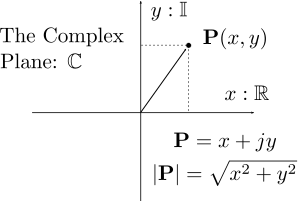
\includegraphics[scale=0.175]{lecture1_fig1.png}


}

% section 3: Stability and the Roots

\section{T3: Finding the Time Value with Time Constant}

\subsection{T3: Finding the Time Value with Time Constant}
\frame{
\frametitle{T3: Finding the Time Value with Time Constant}

In problem b) it asks for the time at which the response equation reaches a certain value. There  are different ways to find this value.

\begin{itemize}
\item Plot the response curve and locate the value graphically. This might not be accurate.\vspc
\item Use a `root-finding' method to locate the value. \vspc
\item Solve for the value with algebra. This is easy for this system.\vspc
\end{itemize}

}

% section 3: Stability and the Roots

\section{T4: Stability of a Second Order System}

\subsection{T4: Stability of a Second Order System}
\frame{
\frametitle{T4: Stability of a Second Order System}


Our model  $m\ddot{x}+c\dot{x}+kx=0$ is stable is the roots of the characteristic equation lie {\it to the right} of the imaginary axis of the complex plane (if the Real part of the root is positive). This makes sense because a positive $\alpha$ would cause the response to go to $\infty$.\vspc

\begin{framed}
This is called the \textbf{Routh-Hurwitz stability conditions}\vspcc

A second order model of the form $a_2s^2+a_1s+a_0=0$ \vspc

if $a_2$, $a_1$, and $a_0$ have the {\it same sign}. \vspc
\end{framed}

This is in your reference handout and discussed on page 488 of System Dynamics, Palm III, Third Edition
}

% references is not a section for now, for looks and it would be a waste of space
\frame{

\frametitle{References}

\begin{itemize}
	\item System Dynamics, Palm III, Third Edition - Chapter 8 - System Response in the Time Domain
\end{itemize}

}
\end{document}









 